% ============================================================
%  VLA track: main body
%  This file replaces vla/mainbody.tex in the supervisor's template.
%  Project: Optimizing Deep Learning on Edge (VLA on Jetson)
%
%  Status labels:
%    [READY]   = Can be written from existing evidence.
%    [PARTIAL] = The method is defined, but final results are pending.p
%    [PENDING] = New experimental evidence is required.
%
%  Workstreams:
%    Method 1 = Runtime-parameter optimisation (PC selection; Jetson validated)
%    Method 2 = Component-wise quantisation (PC selection; Jetson validated)
%    Method 3 = Component-level TensorRT/CUDA Graphs plus connector integration
% ============================================================

% Figures and tables use the document class's default float placement. The
% closing \clearpage prevents VLA floats from entering the next group section.

\section{Optimizing VLA on Edge}

\subsection{Introduction}
% [READY] Approved English draft, updated after the component-level Jetson
% hardware experiments and connector-hybrid ablation.
Vision--Language--Action (VLA) models integrate visual perception and language understanding to generate robot actions from camera observations and natural-language instructions. Representative systems such as RT-2, OpenVLA and SmolVLA illustrate how large-scale vision--language pretraining can be extended to instruction-conditioned robotic manipulation \cite{rt2,openvla,smolvla}. Together with datasets such as Open X-Embodiment, these developments support the construction of increasingly general robot policies \cite{openx}. Deploying such policies directly on robotic platforms, however, requires their computational requirements to be reconciled with the limited resources available on embedded hardware.

Edge deployment involves more than fitting a model into device memory. A practical robotic policy must provide sufficiently low and predictable inference latency while operating within constraints on memory capacity and power consumption. These requirements are closely coupled to control performance, because a slower policy reduces the frequency at which the robot can observe the environment and update its actions. Existing studies have addressed parts of this problem through compact VLA architectures, model compression and visual-token reduction \cite{litevlaedge,nanovla,efficientvla}. Nevertheless, software scheduling, numerical precision and hardware execution are often evaluated separately, leaving their combined effect on end-to-end task performance insufficiently characterised.

A central source of inference cost in SmolVLA is the generation and execution of action sequences. The policy produces actions through iterative flow-matching denoising and supports chunked action prediction \cite{smolvla}. Its deployment cost therefore depends not only on the number of denoising steps, but also on how many actions are predicted and how many are executed before the policy replans. Redundant denoising iterations, frequent replanning and the generation of unused actions can all increase computation \cite{snapflow}. Even after these software-level costs are reduced, operator scheduling and CPU--GPU launch overhead may limit device utilisation \cite{opara}. This motivates a layered optimisation strategy that combines inference-schedule tuning with device-level acceleration using TensorRT and CUDA Graphs \cite{nvidia_tensorrt,nvidia_cuda_graphs}.

Memory pressure creates a complementary deployment constraint. Low-bit weight quantisation offers a direct route to reducing storage and runtime memory, but VLA components need not be equally tolerant of reduced numerical precision. Recent studies have therefore explored saliency-aware, action-guided and hardware-compatible quantisation strategies for VLA policies \cite{sqil,actquant,litevlaedge}. These findings motivate an evaluation that considers both bit width and quantisation scope rather than treating all low-bit configurations as equivalent. Language-only INT8, full-backbone INT8 and mixed 4/8-bit configurations must consequently be compared using task-level success as well as latency and memory measurements.

This study develops a layered optimisation and evaluation pipeline for SmolVLA on the LIBERO benchmark \cite{smolvla,libero}. First, software-level experiments evaluate the joint effects of denoising steps, execution horizon and prediction horizon. A complementary PC-local study then introduces task-aware selection between two execution horizons and a single-retry failure-recovery mechanism. Second, component-wise post-training quantisation is used to examine the trade-off between memory reduction, inference latency and task success. Third, TensorRT engines and CUDA Graph replay are evaluated at the component boundaries supported by the SmolVLA execution path on the Jetson Orin Nano. A TensorRT connector is then reintegrated into the closed-loop policy to test whether component-level acceleration translates into an end-to-end benefit. This design also exposes the practical limits imposed by dynamic model operations, low-bit calibration and device memory. The contribution is therefore a reproducible deployment-optimisation study combining fixed-parameter selection, a task-aware supervisory extension, component-wise quantisation and supported hardware acceleration, rather than a new VLA architecture or a fully compiled VLA runtime.

\subsection{Background and Related Work}
% [READY] Approved English draft based on topic-level synthesis of the
% current literature map. Hardware claims remain bounded to cited sources.
Vision--Language--Action (VLA) models extend vision--language representations to robotic control by conditioning action generation on visual observations, natural-language instructions and, in some cases, robot state. RT-2 formulates robot actions as tokens within a vision--language model, while OpenVLA provides an open-source VLA trained on large-scale robot demonstrations \cite{rt2,openvla}. Octo instead develops a generalist policy using the diverse Open X-Embodiment collection \cite{octo,openx}. Although these models demonstrate the value of large-scale pretraining, their computational requirements complicate embedded deployment. SmolVLA addresses this constraint through a compact vision--language backbone and a flow-matching action expert that predicts chunks of continuous actions \cite{smolvla}. Its combination of a relatively small model, iterative action generation and chunked execution makes it a suitable baseline for studying deployment efficiency without introducing a new policy architecture.

Software-level optimisation can reduce VLA inference cost at several stages of the execution pipeline. For flow-matching policies, each action chunk is generated through repeated denoising, making the number of denoising steps a direct determinant of inference cost. Action chunking introduces an additional trade-off: predicting and executing longer chunks reduces the frequency of policy calls but also increases the interval between observations and replanning \cite{smolvla}. SnapFlow addresses the denoising cost by distilling multi-step flow matching into a one-step action generator, whereas EfficientVLA reduces computation through training-free pruning and visual-token reduction \cite{snapflow,efficientvla}. These approaches demonstrate that action-generation and representation costs can be reduced, but they either modify the learned policy or alter its execution structure. The present study instead begins with inference-time parameters exposed by the released SmolVLA policy, examining denoising-step count, prediction horizon and execution horizon without additional training or architectural modification.

Quantisation provides a complementary route to lower deployment cost by reducing the numerical precision of model weights. However, preserving task-level behaviour under low-bit precision is particularly important for robotic policies, because small numerical perturbations can accumulate through closed-loop execution. SQIL incorporates quantisation into policy fine-tuning and uses saliency-based state importance to protect decisions at mission-critical states \cite{sqil}. ActQuant instead applies action-guided mixed-precision post-training quantisation, allocating precision according to the contribution of individual weight matrices to action prediction \cite{actquant}. LiteVLA-Edge combines 4-bit GGUF quantisation with an accelerated native runtime for fully on-device inference on Jetson Orin-class hardware \cite{litevlaedge}. Collectively, these studies show that bit width alone does not determine deployment quality: the quantisation method, affected model components and runtime support are also consequential. This motivates evaluating both precision and quantisation scope while retaining closed-loop task success alongside latency and memory measurements.

A separate line of work pursues edge deployment through compact architectures or hardware-aware execution. LiteVLA-Edge combines a compact multimodal model with a low-bit runtime, while NanoVLA reduces policy size through decoupled vision--language processing and routing \cite{litevlaedge,nanovla}. These approaches improve deployability by changing the model or its runtime representation. Deployment engines offer another path after model selection. NVIDIA TensorRT compiles supported neural-network components into hardware-specific inference engines and enables graph optimisation and reduced-precision execution \cite{nvidia_tensorrt}. CUDA Graphs capture repeated GPU workloads for replay, reducing the host-side overhead associated with launching many short-running kernels \cite{nvidia_cuda_graphs}. Opara further demonstrates that CUDA Graph construction, stream allocation and operator launch order jointly affect DNN inference efficiency, although its evaluation is not specific to VLA policies or embedded hardware \cite{opara}. The present study evaluates these mechanisms only at compatible SmolVLA component boundaries and separately tests whether an accelerated connector can be reintegrated into closed-loop execution on the Jetson Orin Nano.

Taken together, prior work provides strong evidence for compact VLA architectures, reduced action-generation cost, low-bit quantisation and GPU execution optimisation. These directions are nevertheless commonly evaluated using different policies, runtimes, hardware platforms and task protocols, making their individual and combined effects difficult to separate. This study addresses that evaluation gap by retaining a consistent SmolVLA checkpoint and LIBERO protocol across software-level optimisation, quantisation and on-board validation, while distinguishing standalone component gains from improvements that persist after closed-loop integration.

\subsection{Methodology}

\subsubsection{System and Evaluation Protocol (YH)}
% [PARTIAL] PC-local protocol is complete. Jetson power, temperature and
% utilisation details will be updated after the hardware experiments.
This study considers instruction-conditioned robotic manipulation using SmolVLA on the LIBERO Spatial benchmark \cite{smolvla,libero}. LIBERO defines the language-conditioned tasks, scene assets, initial states and success conditions, while MuJoCo 3.3.2 simulates robot--object dynamics and generates the agent-view and wrist-view observations using EGL off-screen rendering \cite{mujoco}.

At each replanning event, SmolVLA receives the agent-view and wrist-view observations together with a natural-language task instruction and the current robot state. A vision--language backbone processes the visual and linguistic context, and a flow-matching action expert iteratively transforms a noisy trajectory into a sequence of future continuous actions \cite{smolvla}. A selected prefix of this sequence is executed in order by MuJoCo before updated observations trigger the next policy invocation. This repeated observation--prediction--execution cycle provides closed-loop feedback throughout each rollout.

All experiments use the pretrained \texttt{HuggingFaceVLA/smolvla\_libero} checkpoint at revision \texttt{6721902bc4d61e50a3bfdb11dfb4cb626f05d102}. The policy weights are not retrained during this study; instead, the experiments modify its inference schedule, numerical precision and execution runtime. This restriction allows the measured changes in task performance and computational cost to be attributed to deployment-time optimisation rather than additional training or architectural modification.

All rollouts were executed under WSL Ubuntu using Python 3.12.7, LeRobot 0.6.1, HF-LIBERO 0.1.4 and MuJoCo 3.3.2 with EGL rendering. The evaluation pipeline supports both PC-local and edge-deployment configurations. In both configurations, the PC retained responsibility for LIBERO task execution, MuJoCo physics and rendering, environment stepping, success detection, video recording and metric aggregation; only the location of SmolVLA inference was changed. In the PC-local configuration, policy inference ran in the same WSL environment through the official \texttt{lerobot-eval} interface. In the edge-deployment configuration, visual observations, task instructions and robot states were transmitted over HTTP to an NVIDIA Jetson Orin Nano, and the resulting action chunk was returned to the PC for execution in MuJoCo. Both configurations use the same checkpoint, task suite and episode limits. Figure~\ref{fig:vla_system_pipeline} summarises the controlled evaluation routes and layered optimisation pipeline.

\begin{figure}
  \centering
  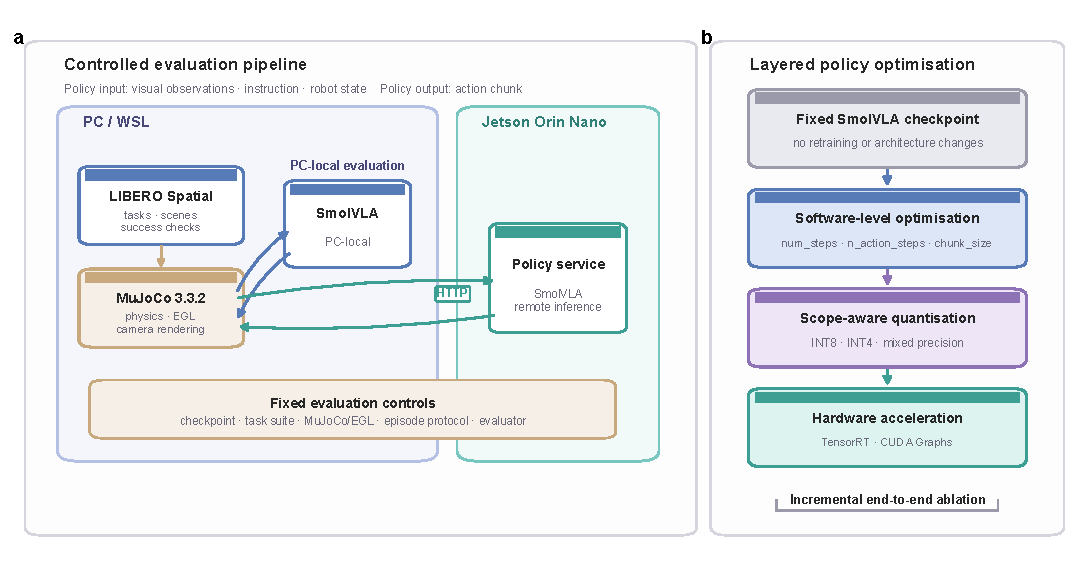
\includegraphics[width=\textwidth]{vla/figures/vla_system_pipeline.pdf}
  \caption{Controlled evaluation and optimisation pipeline for
  SmolVLA. \textbf{a,} PC-local and Jetson inference routes using a common
  LIBERO--MuJoCo evaluation loop. \textbf{b,} Staged evaluation of runtime
  parameters, post-training quantisation, TensorRT and CUDA Graphs, followed
  by an end-to-end ablation.}
  \label{fig:vla_system_pipeline}
\end{figure}

The main fixed-configuration and deployment evaluations use all ten tasks in LIBERO Spatial, with five episodes per task and a maximum episode length of 280 environment steps, giving 50 episodes for each formally reported configuration. The same evaluator settings and random-seed protocol are retained across configurations. Task success is recorded using the binary success signal reported by the official evaluation harness, and uncertainty is represented using Wilson 95\% confidence intervals. Computational performance is characterised using mean and 95th-percentile policy inference latency, mean episode time, parameter memory and peak allocated GPU memory. Because absolute runtime measurements depend on the execution platform, PC and Jetson latency values are interpreted within their respective devices rather than treated as directly interchangeable. Figure~\ref{fig:vla_runtime_parameters}a summarises the observation--prediction--execution cycle used under both deployment routes.

\begin{figure}
  \centering
  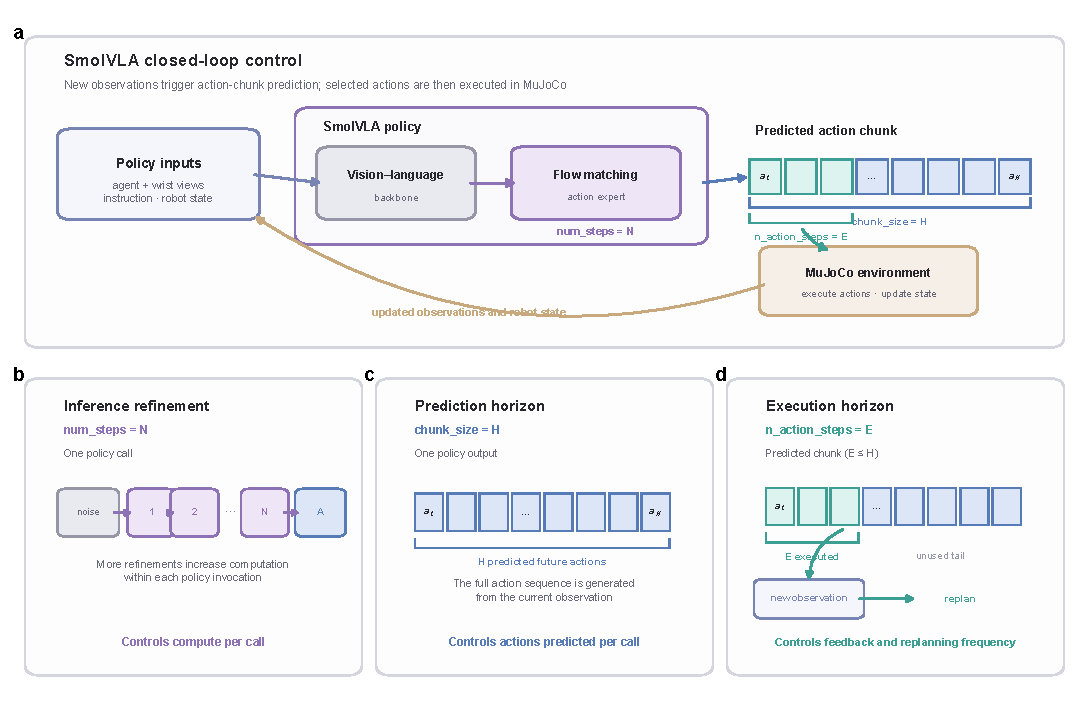
\includegraphics[width=\textwidth]{vla/figures/vla_runtime_parameters.pdf}
  \caption{SmolVLA closed-loop operation and runtime control
  parameters. \textbf{a,} Observation--prediction--execution cycle.
  \textbf{b,} \(N=\texttt{num\_steps}\), the flow-matching refinement depth
  per policy call. \textbf{c,} \(H=\texttt{chunk\_size}\), the predicted
  action horizon. \textbf{d,} \(E=\texttt{n\_action\_steps}\), the executed
  prefix before replanning, where \(1\leq E\leq H\).}
  \label{fig:vla_runtime_parameters}
\end{figure}



\subsubsection{RGB Open-Vocabulary Target Verification (YZ).}
An optional RGB target-verification stage was implemented as a pre-execution safety gate for interactive single-object evaluation. The module rendered a $360\times360$ observation from the LIBERO agent-view camera using the first benchmark initial state. The RGB image and candidate object names were processed by \texttt{IDEA-Research/grounding-dino-tiny}, which associates image regions with textual object descriptions~\cite{liu2024groundingdino}. Detections below a confidence threshold of $0.20$ were removed, followed by class-aware non-maximum suppression with an intersection-over-union threshold of $0.45$.

If the initial query did not return a target-associated label, a second pass used object-specific prompt variants and a confidence threshold no lower than $0.15$. The original RGB frame, annotated predictions, and structured detection records were retained. The detector was then unloaded before SmolVLA was loaded to avoid simultaneous GPU residency.

This RGB module did not provide an additional observation to SmolVLA and was not enabled during the formal LIBERO Spatial or LIBERO Object batch evaluations. Inspection of the saved results identified a failure mode in which the target-specific retry returned a high-confidence bounding box on a non-target region. The module is therefore treated as an exploratory pre-execution safety mechanism rather than a validated target-recognition system. Its outputs were excluded from the formal task-success and latency comparisons.

\begin{figure}[t]
    \centering
    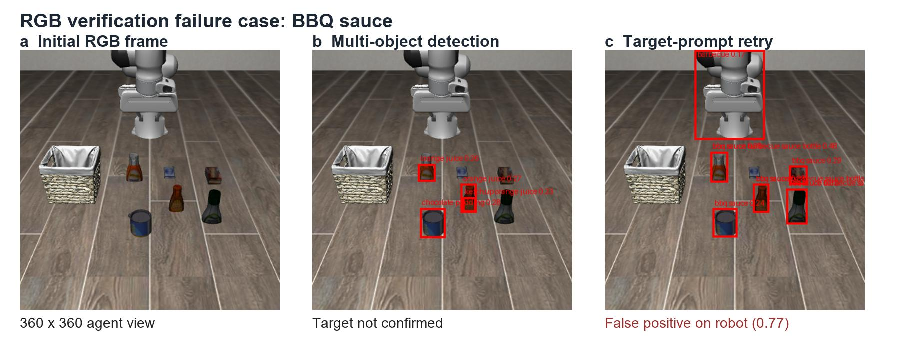
\includegraphics[width=\linewidth]{vla/figures/vla_rgb_failure_case.pdf}
    \caption{Saved BBQ-sauce RGB verification example. The target-specific retry produced a high-confidence prediction on the robot body, demonstrating that a target-associated textual output does not necessarily correspond to spatially correct target localisation.}
    \label{fig:rgb_failure_case}
\end{figure}

\subsubsection{Software-Level Optimisation (YH,YZ)}
% [APPROVED] Section discussed and approved paragraph by paragraph.
Software-level optimisation was performed by varying three inference-time parameters exposed by the released SmolVLA policy while keeping the checkpoint, model weights and evaluation protocol fixed. As illustrated in Fig.~\ref{fig:vla_runtime_parameters}b--d, let \(N\) denote \texttt{num\_steps}, \(H\) denote \texttt{chunk\_size} and \(E\) denote \texttt{n\_action\_steps}. Given observations \(\mathbf{o}_t\), a language instruction \(\mathbf{l}\) and the current robot state \(\mathbf{s}_t\), the policy generates an \(H\)-step action sequence using \(N\) flow-matching refinement iterations:

\begin{equation}
  \mathbf{A}_t =
  F_{\theta}(\mathbf{o}_t,\mathbf{l},\mathbf{s}_t;N,H)
  \in \mathbb{R}^{H\times d_a},
  \qquad
  \operatorname{execute}\!\left(\mathbf{A}_t[1:E]\right),
  \qquad
  1 \leq E \leq H,
  \label{eq:runtime_parameters}
\end{equation}

where \(d_a\) is the action dimension. The evaluator executes the first \(E\) predicted actions before updated observations trigger a new policy call. Consequently, \(N\) controls the computational depth within each policy invocation, \(H\) controls the prediction horizon and \(E\) controls the execution horizon, or equivalently the interval between replanning events.

The refinement-depth experiment used the released inference configuration, \((N,E,H)=(10,1,50)\), with FP16 weights as the baseline. To isolate the effect of refinement depth, \(N\in\{10,5,2\}\) was evaluated while \(E=1\), \(H=50\), the checkpoint, task seeds and evaluator configuration remained fixed. Each setting was evaluated using five episodes for each of the ten LIBERO Spatial tasks, giving 50 episodes per configuration. Task success, mean episode time, and mean and 95th-percentile policy inference latency were recorded to characterise the relationship between flow-matching refinement depth and computational cost.

The execution-horizon experiment fixed \(N=2\) and retained the default prediction horizon \(H=50\), while varying \(E\in\{1,5,10,20,50\}\). Each setting was evaluated over the same 50-episode protocol. Increasing \(E\) allows more actions to be executed from each prediction and therefore reduces the frequency of policy invocation, but it also increases the interval during which the controller acts without incorporating a new observation. The sweep was designed to measure this trade-off rather than assume that either more frequent replanning or longer open-loop execution was uniformly preferable. The \(E=50\) setting additionally tested the limiting case in which the complete predicted action chunk was executed before the next policy call.

A paired prediction-horizon experiment then separated the cost of generating an action sequence from the cost of executing it. With \(N=2\), the default horizon \(H=50\) was compared with a matched horizon \(H=E\) for \(E\in\{1,10,20\}\). The resulting pairs were \((H,E)=(50,1)\) versus \((1,1)\), \((50,10)\) versus \((10,10)\), and \((50,20)\) versus \((20,20)\). Holding the execution horizon fixed within each pair allowed the effect of shortening the predicted sequence to be measured while preserving the replanning interval. When \(H>E\), the actions beyond the executed prefix are discarded after a new observation triggers replanning; setting \(H=E\) removes this unused prediction tail. Because changing the prediction horizon may also affect the generated action sequence, both task success and episode time were retained as evaluation outcomes.

All formally evaluated configurations were compared using task success, mean episode time and policy inference latency. Candidate settings were assessed on the success--time Pareto frontier, with preference given to configurations that reduced runtime without an observed reduction in task success. Wilson 95\% confidence intervals represented uncertainty in the binary success estimates, and differences between overlapping intervals were not interpreted as improved task performance. Quantisation scope was evaluated separately with \(E=1\) and \(H=50\) to isolate precision effects. These fixed-configuration experiments did not use a task-dependent or state-dependent parameter scheduler.

\begin{codexadded}
\subsubsection{Adaptive Execution-Horizon Control (XS)}
\label{sec:xs_adaptive_control}

The adaptive study retained the released SmolVLA prediction chunk at
\(C=50\) actions for every model invocation and changed only the number of
actions executed before replanning. To avoid overloading the existing notation
in Fig.~\ref{fig:vla_runtime_parameters}, the condition labels
\texttt{H1} and \texttt{H20} are treated here as legacy names for execution
horizons \(E=1\) and \(E=20\), respectively; they do not denote the prediction
horizon \(H\) used earlier in this section. Static-H20 executes 20 native
actions, discards actions 21--50 from the fixed prediction chunk, and then
re-observes. Adaptive-v1 and Adaptive-v2a also default to \(E=20\), but a
qualifying trigger truncates the unused active-horizon tail and forces the next
model invocation to execute one action. The following invocation returns to
\(E=20\); for Adaptive-v2a this complete 20-action invocation is a cooldown
before monitoring resumes. Figure~\ref{fig:xs_adaptive_mechanism} summarises
the state transition.

\begin{figure}[!t]
  \centering
  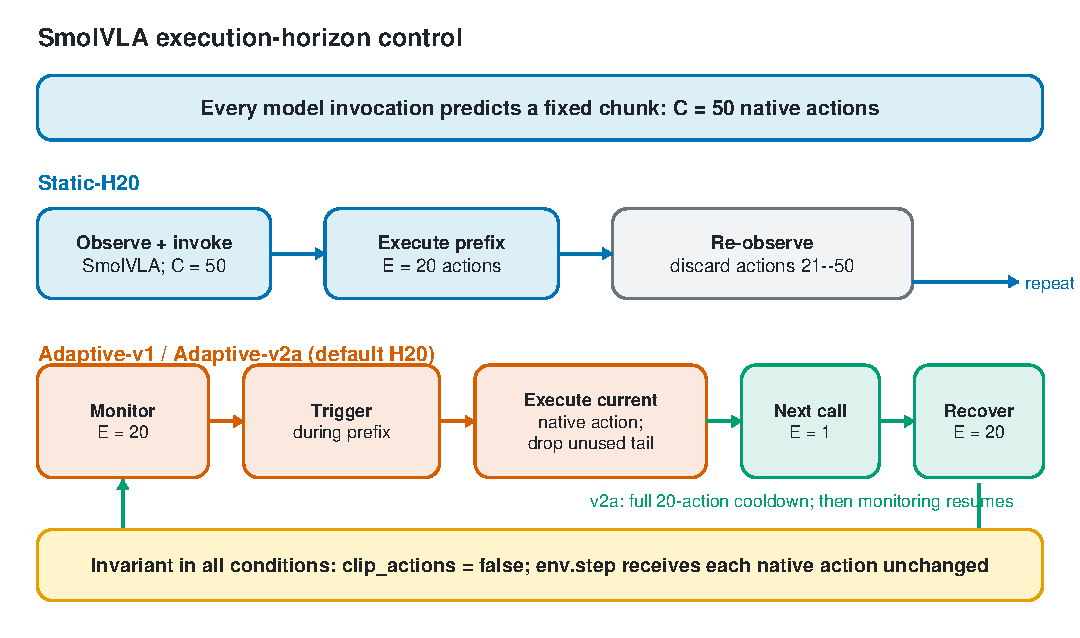
\includegraphics[width=\textwidth]{vla/figures/xs_adaptive/xs_adaptive_mechanism.pdf}
  \codexcaptionsetup
  \caption{\codexfiguretag Descriptive method diagram for the fixed-chunk
  execution controller. Every SmolVLA invocation predicts \(C=50\) actions.
  Static-H20 executes \(E=20\) actions before re-observation. Adaptive-v1 and
  Adaptive-v2a default to \(E=20\); a trigger executes the current native
  action unchanged, discards the unused tail, forces the next invocation to
  \(E=1\), and then recovers to \(E=20\). Adaptive-v2a uses the recovery call
  as a full 20-action cooldown. Action clipping is disabled throughout.}
  \label{fig:xs_adaptive_mechanism}
\end{figure}

\paragraph{Red review note---original-author confirmation requested.}
The existing runtime-parameter figure defines \(H\) as
\texttt{chunk\_size} and \(E\) as \texttt{n\_action\_steps}, whereas the
frozen condition names \texttt{Static-H20} and \texttt{Adaptive-...H20}
use ``H20'' for the execution horizon. The condition names are retained for
provenance, but their captions and first use should continue to state explicitly
that \(C=50\) is the fixed prediction chunk and \(E\in\{1,20\}\) is the
executed prefix.
\end{codexadded}

\subsubsection{Task-Aware Action-Execution Strategy Selection and Failure Recovery (YZ).}
\label{sec:task_aware_routing}
The fixed-configuration sweep identified a single global execution horizon. A
complementary supervisory method instead selected between two horizons using
historical task-level performance. In this independent study,
\(n_{\mathrm{action}}\) denotes the number of predicted actions executed before
replanning and therefore corresponds to the execution horizon \(E\) defined
above. Unlike asynchronous action-prefix alignment methods such as Real-Time
Chunking \cite{rtc}, this method operates only at the task level and does not
modify or retrain the underlying SmolVLA weights. For each LIBERO Object task
\(i\) and
execution strategy \(k\), the historical success probability is estimated
using the Laplace-smoothed score
%
\begin{equation}
    \hat{p}_{i,k}
    =
    \frac{s_{i,k}+1}{n_{i,k}+2},
    \label{eq:laplace_strategy_score}
\end{equation}
%
where \(s_{i,k}\) and \(n_{i,k}\) denote the accumulated numbers of
successful and attempted rollouts, respectively. The strategy with the
highest estimated score is selected before execution. The
\textit{native} configuration retains the checkpoint value
\(n_{\mathrm{action}}=1\), whereas the \textit{smooth} configuration
executes \(n_{\mathrm{action}}=10\) actions before replanning. If both
strategies obtain the same score, the native configuration is selected
as the conservative baseline.

The comparison used all ten tasks in LIBERO Object, with three rollouts per
task, fixed initial states, hard environment resets and a maximum episode
length of 500 control steps. The same random seed was used for both strategies,
giving 30 rollouts per strategy. This protocol was defined independently of the
LIBERO Spatial sweep, so its task-success and rollout-time measurements were
interpreted only within the Native--Smooth comparison.

The proposed hybrid extension additionally monitors the task-level
success signal provided by LIBERO \cite{libero}. When the
initially selected strategy fails, the system automatically switches to
the alternative action horizon and performs one recovery rollout using
a new evaluation seed. Successfully completed tasks are not repeated,
thereby limiting unnecessary computation. The framework records the
initial strategy, historical evidence, recovery strategy, task
completion rate, recovery success rate, execution time, and rollout
videos. The method preserves the original VLA model and maintains a
reproducible separation between baseline, routing and recovery experiments.

\subsubsection{Component-Wise Post-Training Quantisation (YH)}
% [APPROVED] Formal configurations only; mixed precision was verified from the
% original run command as vision INT4, connector INT4 and text INT8.
Component-wise weight-only post-training quantisation (PTQ) was applied when loading the pretrained SmolVLA checkpoint to reduce its deployment memory requirements without additional training. The original checkpoint was loaded through an inference-only policy wrapper, after which selected linear layers in the vision--language backbone were replaced by quantised equivalents. No gradient updates, fine-tuning data or activation-calibration dataset were used. The flow-matching action expert, embedding layers and output heads remained in FP16, preserving the original action-generation and action-queue semantics. This design isolates the effects of numerical precision and quantisation scope without modifying the policy architecture or closed-loop execution procedure.

Each targeted weight matrix was partitioned along its input dimension into groups of 128 values and quantised using symmetric group-wise absolute-maximum scaling. For a weight group \(\mathbf{w}_g\) and bit width \(b\), the scale and quantised values were computed as

\begin{equation}
  s_g=\frac{\max_i |w_{g,i}|}{2^{b-1}-1},
  \qquad
  q_{g,i}=\operatorname{clip}\!\left(
    \operatorname{round}\!\left(\frac{w_{g,i}}{s_g}\right),
    -\left(2^{b-1}-1\right),
    2^{b-1}-1
  \right).
  \label{eq:groupwise_quantisation}
\end{equation}

The approximate weight used for inference is therefore \(\hat{w}_{g,i}=s_gq_{g,i}\). INT8 weights were stored as signed 8-bit integers with one FP32 scale per group, whereas pairs of signed INT4 values were packed into \texttt{uint8} storage with the corresponding FP32 scales. During each forward pass, the stored weights were dequantised to the input tensor data type before the linear operation. Activation precision and the original automatic mixed-precision execution path were retained. The implementation consequently targets parameter-storage and GPU-memory reduction rather than native low-bit arithmetic, making empirical latency measurement necessary.

Four formally evaluated precision configurations were defined, as summarised in Table~\ref{tab:quantisation_configurations}.

\begin{table}
  \centering
  \caption{Component-wise precision configurations used in the formal
  quantisation experiments. \(N\) denotes \texttt{num\_steps}. Embedding layers
  and output heads retain their original precision in every configuration.}
  \label{tab:quantisation_configurations}
  \small
  \begin{tabular}{@{}lcccccc@{}}
    \toprule
    Configuration & Vision & Connector & Text & Action expert & \(N\) \\
    \midrule
    FP16 baseline       & FP16 & FP16 & FP16 & FP16 & 10, 2 \\
    Language-only INT8  & FP16 & FP16 & INT8 & FP16 & 10, 2 \\
    Backbone INT8       & INT8 & INT8 & INT8 & FP16 & 10, 2 \\
    Mixed 4/8-bit       & INT4 & INT4 & INT8 & FP16 & 2 \\
    \bottomrule
  \end{tabular}
\end{table}

The language-only configuration quantised the linear layers of the text transformer while preserving the vision encoder and multimodal connector in FP16. The backbone configuration extended INT8 quantisation to the vision encoder, connector and text transformer. The mixed configuration instead assigned INT4 weights to the vision encoder and connector while retaining the text transformer at INT8. The action expert remained in FP16 in every configuration, allowing the experiment to compare the memory and computational effects of reducing precision in different parts of the vision--language backbone.

Two additional INT4 probes were used to identify a low-bit component-sensitivity boundary. One quantised only the text transformer to INT4, whereas the other quantised the vision encoder, connector and text transformer to INT4; the action expert, embeddings and output heads again remained in FP16. These probes used one episode for each LIBERO Spatial task at \(N=10\) and were excluded from the formal configuration-ranking protocol. They therefore provide contextual evidence for interpreting the mixed 4/8-bit configuration rather than a statistically comparable alternative.

Quantisation was evaluated on LIBERO Spatial using the same SmolVLA checkpoint revision and evaluator configuration as the software-level experiments. The execution horizon and prediction horizon were fixed at \(E=1\) and \(H=50\), respectively. FP16, language-only INT8 and backbone INT8 were evaluated at \(N\in\{10,2\}\), whereas the mixed configuration was evaluated at \(N=2\). Each formal configuration comprised five episodes for each of the ten tasks, giving 50 episodes per configuration. Closed-loop task success was measured using the simulator evaluation, while a separate policy-only benchmark recorded mean and 95th-percentile inference latency, stored parameter size and peak allocated GPU memory. Candidate configurations were selected according to the joint trade-off between task success, memory use and latency. Because the custom layers perform forward-time dequantisation followed by floating-point linear operations, these PC measurements were not treated as evidence of hardware-native INT8 acceleration.

% [VERIFY BEFORE SUBMISSION] Preserve the exact policy-only benchmark invocation
% and raw log before reporting warm-up and timed-iteration counts in the paper.

\subsubsection{Component-Level Hardware Acceleration (YH)}

Hardware-specific evaluation was conducted on the Jetson Orin Nano using the
same SmolVLA checkpoint revision as the preceding experiments. The software
environment used L4T R36.4.4, TensorRT 10.11.0 and ONNX 1.17.0. To preserve
the released policy architecture while isolating hardware-execution effects,
the vision encoder and multimodal connector were treated as separate
acceleration boundaries. Components outside the active TensorRT boundary
continued to execute through the original PyTorch policy. Standalone engine
benchmarks and closed-loop policy evaluation were retained as distinct
measurement levels.

\begin{table}
  \centering
  \caption{Component-level hardware-acceleration experiment design. Input
  specifications are fixed for each engine and are not compared across rows.}
  \label{tab:hardware_experiment_design}
  \small
  \setlength{\tabcolsep}{3pt}
  \renewcommand{\arraystretch}{1.12}
  \begin{tabular}{@{}p{0.20\textwidth}p{0.17\textwidth}p{0.27\textwidth}p{0.25\textwidth}@{}}
    \toprule
    Experiment & Scope & Precision and fixed input & Evaluation level \\
    \midrule
    Connector probe & Connector & FP16; 256 visual tokens & Standalone engine \\
    Connector hybrid & Connector & FP16; 1,024 visual tokens & Closed-loop rollout \\
    Vision FP16 & Vision encoder & FP16; \(256\times256\) image & Standalone and hybrid \\
    Vision INT8 & Vision encoder & Calibrated INT8; \(512\times512\) image & Standalone and hybrid \\
    CUDA Graphs & FP16 vision engine & Fixed engine input & Eager enqueue versus graph replay \\
    \bottomrule
  \end{tabular}
\end{table}

The connector and vision encoder were exported with \texttt{torch.onnx.export}
using ONNX opset 17. The vision encoder export used the dynamo exporter, eager
attention and a fixed batch size of one; its patch-attention mask was embedded
in the exported graph. The fixed input specifications are summarised in
Table~\ref{tab:hardware_experiment_design}. FP16 engines were built with
\texttt{trtexec}. For the INT8 vision path, an entropy calibrator consumed up
to 400 saved LIBERO image tensors with batch size one; the TensorRT builder
used explicit-batch mode, optimisation level one and a 128-MiB workspace
limit.

Component latency was measured after a warm-up phase using identical timing
settings within each paired comparison. The predefined metrics were mean and
95th-percentile GPU latency and throughput. CUDA Graphs were evaluated on the
same FP16 TensorRT vision engine by comparing conventional eager enqueue with
graph replay under fixed inputs. Enqueue time was recorded separately from GPU
execution latency \cite{nvidia_tensorrt,nvidia_cuda_graphs}. For hybrid
evaluation, the engine wrapper preallocated and bound GPU tensors, launched
asynchronously on the current CUDA stream and replaced the corresponding
PyTorch module. The remaining policy and the LIBERO--MuJoCo evaluation loop
were held constant. Component latency was not treated as closed-loop policy
latency.

% [VERIFY BEFORE SUBMISSION] Recover the exact TensorRT warm-up and timed-run
% counts from the Jetson command log before adding them to the visible prose.

\subsubsection{Incremental On-Board Ablation (YH)}

\begin{table}
  \centering
  \caption{Incremental on-board ablation design. All configurations use
  \((N,E,H)=(2,20,20)\); the vision encoder and action expert remain in FP16.}
  \label{tab:onboard_ablation_design}
  \small
  \setlength{\tabcolsep}{4pt}
  \begin{tabular}{@{}p{0.25\textwidth}p{0.18\textwidth}p{0.22\textwidth}p{0.22\textwidth}@{}}
    \toprule
    Configuration & Runtime parameters & Text transformer & Connector \\
    \midrule
    Software FP16 & \((2,20,20)\) & FP16 & PyTorch FP16 \\
    Software + INT8 & \((2,20,20)\) & Group-wise INT8 & PyTorch FP16 \\
    Software + INT8 + TRT & \((2,20,20)\) & Group-wise INT8 & TensorRT FP16 \\
    \bottomrule
  \end{tabular}
\end{table}

The three configurations used the same Jetson device, checkpoint revision,
remote evaluation route and ten LIBERO Spatial tasks. Five episodes were
evaluated for each task, giving 50 episodes per configuration. Task success was
recorded as a binary outcome and summarised as a point estimate with a Wilson
95\% confidence interval. Mean episode time was calculated over the complete
rollout set, while mean policy-inference latency and the number of prediction
requests were obtained from the request-level service traces. Component-engine
latencies were excluded from these closed-loop metrics, ensuring that each
ablation comparison reflected the complete policy execution path. TensorRT
vision execution and CUDA Graph replay were evaluated separately and were not
additional factors in this ablation.

% [VERIFY BEFORE SUBMISSION] Archive the TensorRT-connector run's eval_info.json
% and remote_transport.jsonl before reporting its confidence interval and
% request-level statistics in Section 4.5.


\subsection{Experimental Results}

\subsubsection{PC-Local Software-Level Optimisation (YH,YZ)}
% [APPROVED/WRITTEN] Prose, numerical tables and Figure 3 approved and inserted.

PC-local evaluation showed that the three runtime parameters affected different
sources of computational cost, with flow-matching refinement depth providing the
largest individual reduction in runtime. Each formal configuration was evaluated
over 50 LIBERO Spatial episodes, comprising five episodes for each of the ten
tasks. Figure~\ref{fig:software_optimization} visualises the resulting trade-offs,
while Tables~\ref{tab:pc_refinement_depth}--\ref{tab:pc_prediction_matching}
provide the corresponding numerical results.

\begin{figure}[!t]
  \centering
  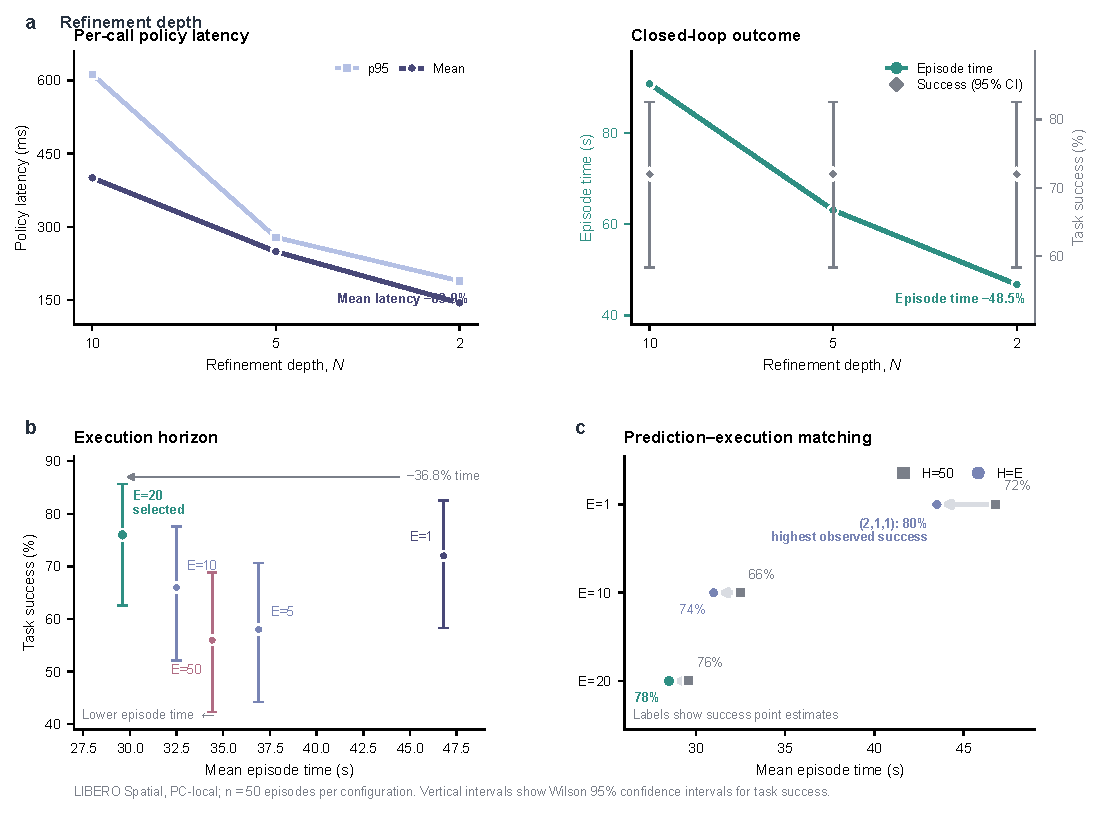
\includegraphics[width=0.92\textwidth]{vla/figures/vla_software_optimization.pdf}
  \caption{PC-local software-level optimisation of SmolVLA on LIBERO Spatial.
  \textbf{a,} Flow-matching refinement depth \(N\), with \(E=1\) and \(H=50\).
  \textbf{b,} Execution-horizon trade-off, with \(N=2\) and \(H=50\).
  \textbf{c,} Released \(H=50\) versus matched \(H=E\), with \(N=2\).
  Highlighted labels mark the highest observed success point \((2,1,1)\) and
  the selected time--success trade-off \((2,20,20)\). Error bars are Wilson
  95\% confidence intervals; each configuration contains 50 episodes.}
  \label{fig:software_optimization}
\end{figure}

Reducing the refinement depth \(N\) substantially decreased both policy latency
and episode time (Fig.~\ref{fig:software_optimization}a and
Table~\ref{tab:pc_refinement_depth}). All three tested settings achieved a
task-success rate of 72.0\%. Reducing \(N\) from 10 to 2 lowered mean policy
latency by 63.9\% and mean episode time by 48.5\%, without an observed reduction
in task success. The \(N=2\) setting was therefore retained for the subsequent
parameter sweeps.

\begin{table}
  \centering
  \caption{Flow-matching refinement-depth sweep on LIBERO Spatial, with \(E=1\)
  and \(H=50\). Each configuration contains 50 episodes. Arrows indicate the
  preferred direction of each metric.}
  \label{tab:pc_refinement_depth}
  \small
  \setlength{\tabcolsep}{4pt}
  \begin{tabular}{@{}ccccc@{}}
    \toprule
    \(N\) & Success (\%) \(\uparrow\) &
    \shortstack{Mean latency\\(ms) \(\downarrow\)} &
    \shortstack{p95 latency\\(ms) \(\downarrow\)} &
    \shortstack{Episode time\\(s) \(\downarrow\)} \\
    \midrule
    10 & 72.0 & 400.4 & 612.1 & 90.8 \\
    5  & 72.0 & 249.3 & 278.6 & 63.1 \\
    \textbf{2} & 72.0 & \textbf{144.6} & \textbf{189.4} &
    \textbf{46.8} \\
    \bottomrule
  \end{tabular}
\end{table}

After fixing \(N=2\), the execution horizon \(E\) exhibited a non-monotonic
success--time trade-off (Fig.~\ref{fig:software_optimization}b and
Table~\ref{tab:pc_execution_horizon}). Increasing \(E\) from 1 to 20 reduced
mean episode time from 46.8 to 29.6\,s, while the observed success rate changed
from 72.0\% to 76.0\%. Extending the horizon to \(E=50\) did not provide a further
benefit: both episode time and the success-rate point estimate deteriorated
relative to \(E=20\). The \(E=20\) configuration therefore provided the most
favourable observed operating point in this sweep. Overlapping confidence
intervals do not support interpreting its higher success-rate point estimate as
improved task capability.

\begin{table}
  \centering
  \caption{Execution-horizon sweep on LIBERO Spatial, with \(N=2\) and \(H=50\).
  Each configuration contains 50 episodes. Arrows indicate the preferred
  direction of each metric.}
  \label{tab:pc_execution_horizon}
  \small
  \begin{tabular}{@{}ccc@{}}
    \toprule
    \(E\) & Success (\%) \(\uparrow\) & Episode time (s) \(\downarrow\) \\
    \midrule
    1  & 72.0 & 46.8 \\
    5  & 58.0 & 36.9 \\
    10 & 66.0 & 32.5 \\
    \textbf{20} & \textbf{76.0} & \textbf{29.6} \\
    50 & 56.0 & 34.4 \\
    \bottomrule
  \end{tabular}
\end{table}

Matching the prediction horizon \(H\) to the execution horizon \(E\) provided a
smaller additional reduction in episode time (Fig.~\ref{fig:software_optimization}c
and Table~\ref{tab:pc_prediction_matching}). Across the three evaluated pairs,
replacing \(H=50\) with \(H=E\) reduced mean episode time by 3.7--7.1\%, without a
lower observed success-rate point estimate. The \((N,E,H)=(2,1,1)\) configuration
achieved the highest observed success rate of 80.0\%, but required 43.5\,s per
episode. In comparison, \((2,20,20)\) achieved 78.0\% success with a mean episode
time of 28.5\,s. The latter was therefore selected as the fixed software
configuration.

\begin{table}
  \centering
  \caption{Prediction-horizon matching on LIBERO Spatial, comparing the released
  horizon \(H=50\) with \(H=E\) at fixed \(N=2\). Each configuration contains
  50 episodes.}
  \label{tab:pc_prediction_matching}
  \small
  \setlength{\tabcolsep}{4pt}
  \begin{tabular}{@{}cccccc@{}}
    \toprule
    \(E\) & \shortstack{Success\\\(H=50\) (\%)} &
    \shortstack{Time\\\(H=50\) (s)} &
    \shortstack{Success\\\(H=E\) (\%)} &
    \shortstack{Time\\\(H=E\) (s)} & Time change \\
    \midrule
    1  & 72.0 & 46.8 & \textbf{80.0} & 43.5 & -7.1\% \\
    10 & 66.0 & 32.5 & 74.0 & 31.0 & -4.6\% \\
    \textbf{20} & 76.0 & 29.6 & \textbf{78.0} & \textbf{28.5} & -3.7\% \\
    \bottomrule
  \end{tabular}
\end{table}

Relative to the released \((10,1,50)\) configuration in
Table~\ref{tab:pc_refinement_depth}, the selected \((2,20,20)\) configuration in
Table~\ref{tab:pc_prediction_matching} reduced mean episode
time by 68.6\%, from 90.8 to 28.5\,s. Its success-rate point estimate changed
from 72.0\% to 78.0\%; however, the corresponding Wilson 95\% confidence
intervals---58.3--82.5\% and 64.8--87.2\%, respectively---overlapped. The result
therefore supports substantially lower PC-local runtime without an observed loss
of task performance, rather than improved task capability. These findings support
a fixed operating point under the evaluated LIBERO Spatial protocol, but do not
establish the benefit of task-dependent parameter adaptation.

\begin{codexadded}
\subsubsection{Adaptive Success--Compute Trade-off (XS)}
\label{sec:xs_adaptive_results}

Figure~\ref{fig:xs_success_compute_tradeoff} reports the frozen relationship
between Success@280 and computation without pooling cohorts. In the
parity-corrected development cohort, Static-H1, Static-H10, Static-H20 and
Adaptive-v1 achieved \(33/50\), \(30/50\), \(32/50\) and \(31/50\)
successes, with 162.48, 17.48, 8.66 and 9.08 mean model invocations per
episode, respectively. The paired Adaptive-v1 minus Static-H20 success
difference was \(-0.02\) (task-cluster bootstrap 95\% CI
\([-0.06,0.00]\); exact two-sided McNemar \(p=1.0\)), while the mean model-call
difference was \(+0.42\) (95\% CI \([0.08,0.90]\)). Seven development
triggers produced no rescues, one loss and six no-change events; these results
are descriptive development evidence rather than held-out confirmation.

In the untouched held-out confirmatory cohort, Static-H20 and Adaptive-v2a
both achieved \(33/50\) successes, with 8.32 and 8.36 mean model invocations
per episode. Their paired success difference was exactly 0.00 in this sample
(95\% CI \([0.00,0.00]\); McNemar \(p=1.0\)); Adaptive-v2a used 0.04 more
model calls per episode on average (95\% CI \([0.00,0.12]\)). The single
held-out trigger completed the full \(E20\!\rightarrow\!E1\!\rightarrow\!E20\)
state chain but did not change the paired success outcome. Equal point
estimates are not interpreted as a non-inferiority result, and no statistic is
computed across the two cohorts.

\begin{figure}[!t]
  \centering
  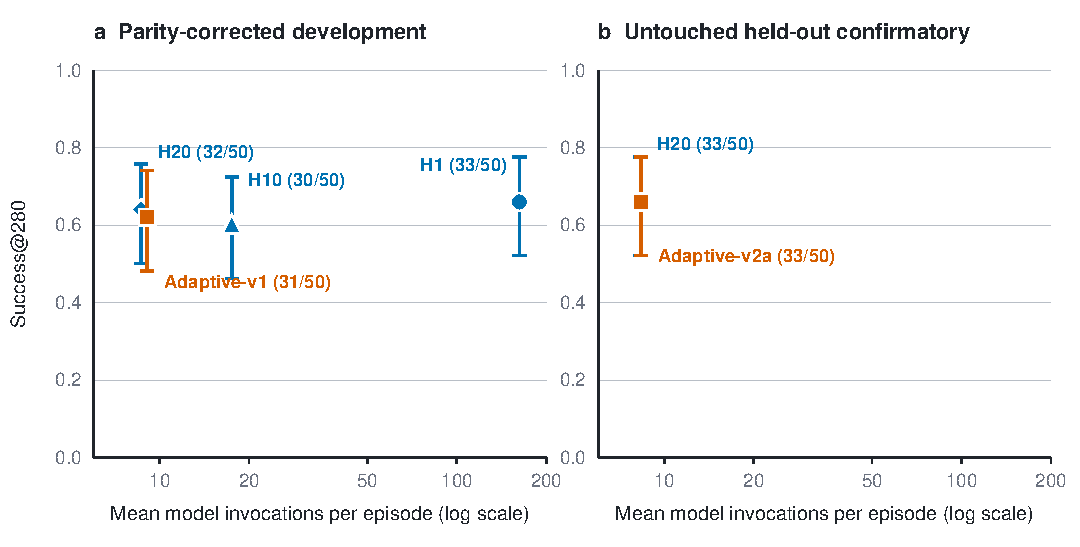
\includegraphics[width=\textwidth]{vla/figures/xs_adaptive/xs_success_compute_tradeoff.pdf}
  \codexcaptionsetup
  \caption{\codexfiguretag Success--compute trade-off from the frozen final
  VLA results. The x-axis is mean model invocations per episode (log scale) and
  the y-axis is Success@280 over its full \([0,1]\) range; labels give
  successes out of 50 and vertical intervals are Wilson 95\% confidence
  intervals. \textbf{a,} Descriptive parity-corrected development results for
  H1, H10, H20 and Adaptive-v1; paired comparisons are computed only within
  this cohort. \textbf{b,} Preregistered paired results for Static-H20 and
  Adaptive-v2a in the untouched held-out confirmatory cohort. The panels are
  not pooled, and early evaluator-parity results are excluded.}
  \label{fig:xs_success_compute_tradeoff}
\end{figure}
\end{codexadded}

\paragraph{Independent Native--Smooth Evaluation on LIBERO Object (YZ).}
The native and smooth action-execution strategies were compared under the
independent protocol defined in Section~\ref{sec:task_aware_routing}. The native
strategy completed 22 of 30 rollouts, corresponding to a success rate of
$73.33\%$. It required 5938.33~s in total, or 197.94~s per rollout. The smooth
strategy completed 24 of 30 rollouts, corresponding to a success rate of
$80.00\%$, and required 1111.58~s in total, or 37.05~s per rollout.

The smooth strategy therefore reduced mean rollout time by $81.3\%$, corresponding to a 5.34-fold speed-up. Its success-rate point estimate was 6.67 percentage points higher than that of the native strategy. However, because each strategy contained only 30 rollouts, the difference in success rate is treated as a descriptive result and is not interpreted as a statistically significant improvement.

\begin{figure*}[t]
    \centering
    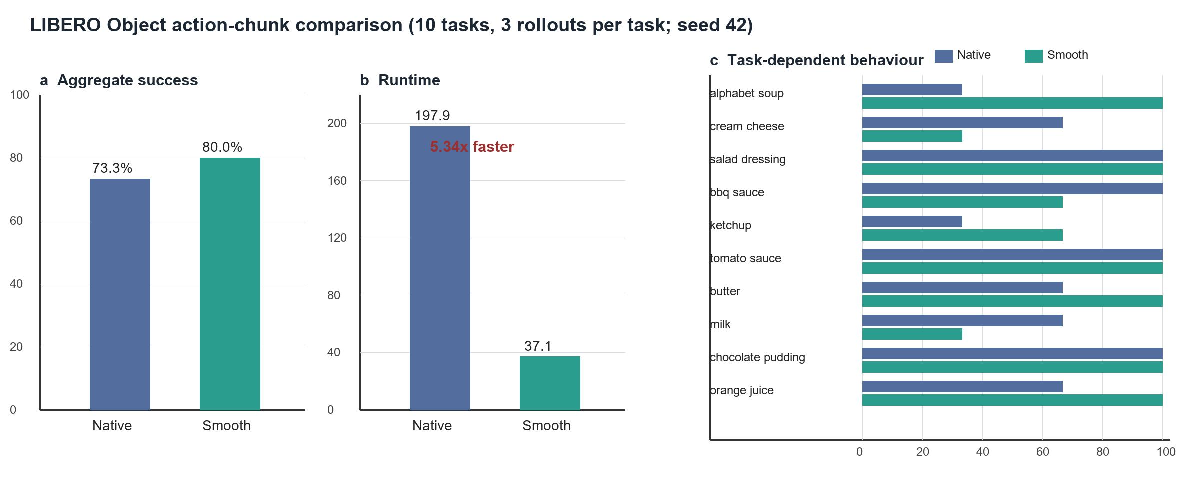
\includegraphics[width=0.96\textwidth]{vla/figures/vla_action_chunk_results.pdf}
    \caption{Independent comparison of the Native and Smooth action-execution strategies on LIBERO Object. Aggregate success and runtime results are accompanied by per-task success rates. Each strategy contains 30 rollouts: three rollouts for each of ten tasks using seed 42.}
    \label{fig:vla_action_execution_results}
\end{figure*}

As shown in Fig.~\ref{fig:vla_action_execution_results}, the aggregate results concealed task-level variation. The native strategy performed better for cream cheese, BBQ sauce, and milk, whereas the smooth strategy performed better for alphabet soup, ketchup, butter, and orange juice. The two strategies produced equal results for salad dressing, tomato sauce, and chocolate pudding. These results indicate that a single action-execution strategy was not optimal for every object category and provide the experimental motivation for task-aware execution-strategy selection.

The exploratory router runs covered different task subsets and evaluation protocols. Their outcomes were therefore not pooled with the matched Native--Smooth experiment and are not presented as evidence that routing outperformed the best fixed strategy.

Because the benchmark suite, episode horizon and sampling protocol differed
from the LIBERO Spatial sweep, these rollout times are interpreted only within
the Native--Smooth comparison and are not compared numerically with the Spatial
or Jetson latency measurements reported below. The success percentages are
treated as descriptive point estimates. This complementary experiment motivates
task-aware routing but was not used to select the fixed configuration deployed
in the subsequent Jetson experiments.

\subsubsection{PC-Local Component-Wise Quantisation (YH)}
% [APPROVED/WRITTEN; FIGURE INSERTED] The prose, Fig. 5 and Tables 7--9 follow
% the approved five-paragraph structure.

Component-wise post-training quantisation reduced stored parameter size and peak
allocated GPU memory, whereas its effect on PC-local policy latency depended on
quantisation scope. Quantisation scope was screened independently of the
execution- and prediction-horizon candidate selected by the software-level
sweep: \(E=1\) and \(H=50\) were retained throughout this comparison.
Closed-loop task success was evaluated at \(N=10\) and \(N=2\). The former
provided a reference under the released refinement depth, whereas the latter
represented the refinement depth retained for optimisation. Each reported closed-loop configuration
comprised 50 LIBERO Spatial episodes. For candidate selection, a policy-only
benchmark compared all four precision configurations at \(N=2\), measuring mean
and 95th-percentile latency, stored parameter size and peak allocated GPU memory.
Figure~\ref{fig:quantisation_results} visualises the success, latency, memory and
candidate trade-offs, while Tables~\ref{tab:pc_quant_success},
\ref{tab:pc_int4_probes} and \ref{tab:pc_quant_benchmark} provide the
corresponding numerical results.

\begin{figure}[!t]
  \centering
  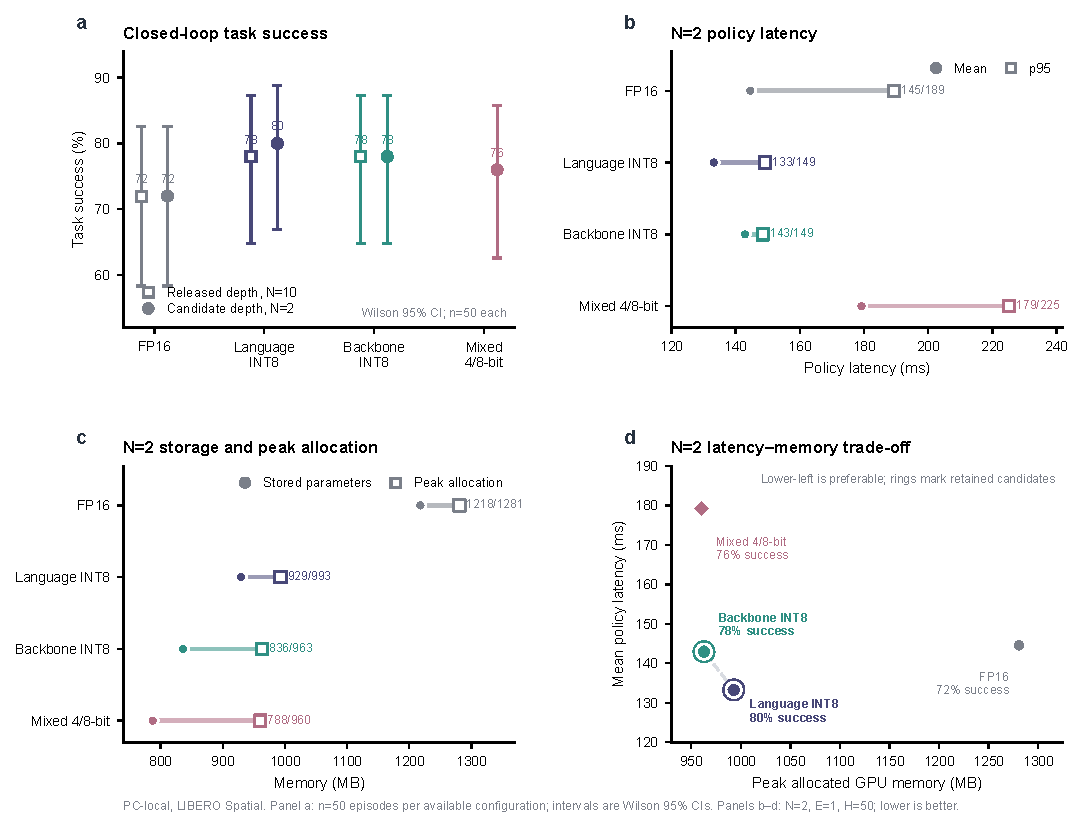
\includegraphics[width=0.92\textwidth]{vla/figures/vla_quantisation_results.pdf}
  \caption{PC-local component-wise post-training quantisation of SmolVLA on
  LIBERO Spatial. \textbf{a,} Task success at \(N=10\) and \(N=2\); error bars
  are Wilson 95\% confidence intervals (50 episodes per available
  configuration). \textbf{b,} Mean and 95th-percentile policy latency.
  \textbf{c,} Stored parameter size and peak allocated GPU memory.
  \textbf{d,} Latency--memory trade-off, with success point estimates and
  retained candidates marked by rings. Panels b--d use \(N=2\), \(E=1\) and
  \(H=50\).}
  \label{fig:quantisation_results}
\end{figure}

Task-success point estimates did not show a loss under any evaluated
quantisation scope (Fig.~\ref{fig:quantisation_results}a and
Table~\ref{tab:pc_quant_success}). At \(N=10\), the FP16
baseline achieved 72.0\% success, whereas both language-only INT8 and backbone
INT8 achieved 78.0\%. At \(N=2\), the corresponding point estimates were
72.0\%, 80.0\% and 78.0\%, and the mixed 4/8-bit configuration achieved
76.0\%. The Wilson 95\% confidence intervals overlapped across all
configurations, providing no evidence of either improved or reduced task
capability under the evaluated quantisation settings.

\begin{table}
  \centering
  \caption{Closed-loop task success for the formal PC-local quantisation
  configurations on LIBERO Spatial. Results at the released refinement depth
  \(N=10\) are shown alongside the candidate refinement depth \(N=2\). Each
  available entry contains 50 episodes; dashes indicate an unevaluated
  configuration. Confidence intervals are Wilson 95\% intervals for binary
  task success.}
  \label{tab:pc_quant_success}
  \small
  \setlength{\tabcolsep}{4pt}
  \begin{tabular}{@{}lcccc@{}}
    \toprule
    & \multicolumn{2}{c}{Released depth, \(N=10\)} &
      \multicolumn{2}{c}{Candidate depth, \(N=2\)} \\
    \cmidrule(lr){2-3}\cmidrule(lr){4-5}
    Configuration &
    \shortstack{Success\\(\%) \(\uparrow\)} &
    \shortstack{Wilson 95\%\\CI (\%)} &
    \shortstack{Success\\(\%) \(\uparrow\)} &
    \shortstack{Wilson 95\%\\CI (\%)} \\
    \midrule
    FP16 baseline      & 72.0 & 58.3--82.5 & 72.0 & 58.3--82.5 \\
    Language-only INT8 & 78.0 & 64.8--87.2 & \textbf{80.0} & 67.0--88.8 \\
    Backbone INT8      & 78.0 & 64.8--87.2 & 78.0 & 64.8--87.2 \\
    Mixed 4/8-bit      & --   & --         & 76.0 & 62.6--85.7 \\
    \bottomrule
  \end{tabular}
\end{table}

Exploratory INT4 probes exposed a component-dependent precision boundary
(Table~\ref{tab:pc_int4_probes}). At \(N=10\), quantising only the text
transformer to INT4 yielded 10.0\% success over ten episodes, while quantising
the vision encoder, connector and text transformer to INT4 yielded 30.0\%.
These probes were not used for configuration-level ranking because each task
was sampled once. Nevertheless, they contrast with the 76.0\% success of the
formal mixed 4/8-bit configuration, in which the vision encoder and connector
were INT4 but the text transformer remained INT8. This pattern suggests that
the text transformer is more sensitive to 4-bit quantisation in this system;
it does not isolate the vision encoder and connector individually or test the
action expert below FP16.

\begin{table}
  \centering
  \caption{Exploratory low-bit component-sensitivity probes, shown alongside
  the formal mixed 4/8-bit configuration. The action expert, embedding layers
  and output heads remained FP16. The INT4 probes used one episode for each
  LIBERO Spatial task and were not used for formal configuration ranking.}
  \label{tab:pc_int4_probes}
  \small
  \setlength{\tabcolsep}{3.5pt}
  \begin{tabular}{@{}lcccccc@{}}
    \toprule
    Configuration & Vision & Connector & Text & \(N\) & Episodes &
    \shortstack{Success\\(\%)} \\
    \midrule
    Text-only INT4 probe & FP16 & FP16 & INT4 & 10 & 10 & 10.0 \\
    Backbone INT4 probe & INT4 & INT4 & INT4 & 10 & 10 & 30.0 \\
    Mixed 4/8-bit (formal) & INT4 & INT4 & INT8 & 2 & 50 & 76.0 \\
    \bottomrule
  \end{tabular}
\end{table}

The memory benefit increased as quantisation was extended across the
vision--language backbone (Fig.~\ref{fig:quantisation_results}c). Relative to
the 1217.9\,MB FP16 parameter footprint,
language-only INT8 reduced stored parameter size by 23.7\% to 929.4\,MB,
backbone INT8 reduced it by 31.4\% to 835.9\,MB, and mixed 4/8-bit reduced it by
35.3\% to 787.5\,MB. Peak allocated GPU memory decreased from 1280.8\,MB for
FP16 to 992.9\,MB, 962.8\,MB and 960.1\,MB, respectively, corresponding to
reductions of 22.5\%, 24.8\% and 25.0\%. Thus, broadening the quantised scope
continued to reduce stored parameter size, but the additional reduction in peak
GPU allocation became small beyond language-only INT8.

Policy latency showed a different scope-dependent pattern
(Fig.~\ref{fig:quantisation_results}b and
Table~\ref{tab:pc_quant_benchmark}). At \(N=2\), language-only INT8 reduced
mean latency from 144.57 to 133.25\,ms and p95 latency from 189.36 to
149.22\,ms, corresponding to reductions of 7.8\% and 21.2\%, respectively.
Backbone INT8 produced a smaller 1.1\% reduction in mean latency, to
142.93\,ms, while reducing p95 latency by 21.6\% to 148.52\,ms. In contrast,
mixed 4/8-bit increased mean and p95 latency by 24.0\% and 19.0\%, to 179.21
and 225.26\,ms. Greater parameter compression therefore did not translate
monotonically into lower latency in the custom PC-local execution path.

\begin{table}
  \centering
  \caption{Policy-only PC-local benchmark used for quantisation candidate
  selection, with \(N=2\), \(E=1\) and \(H=50\). Arrows indicate the preferred
  direction of each metric.}
  \label{tab:pc_quant_benchmark}
  \small
  \setlength{\tabcolsep}{4pt}
  \begin{tabular}{@{}lcccc@{}}
    \toprule
    Configuration &
    \shortstack{Mean latency\\(ms) \(\downarrow\)} &
    \shortstack{p95 latency\\(ms) \(\downarrow\)} &
    \shortstack{Stored parameter\\size (MB) \(\downarrow\)} &
    \shortstack{Peak memory\\(MB) \(\downarrow\)} \\
    \midrule
    FP16 baseline      & 144.6 & 189.4 & 1217.9 & 1280.8 \\
    Language-only INT8 & \textbf{133.3} & 149.2 & 929.4 & 992.9 \\
    Backbone INT8      & 142.9 & \textbf{148.5} & 835.9 & 962.8 \\
    Mixed 4/8-bit      & 179.2 & 225.3 & \textbf{787.5} & \textbf{960.1} \\
    \bottomrule
  \end{tabular}
\end{table}

No single quantised configuration dominated the \(N=2\) comparison
(Fig.~\ref{fig:quantisation_results}d). The language-only INT8 configuration
was retained as the performance-oriented
candidate because it combined the lowest mean latency with the highest observed
success-rate point estimate. Backbone INT8 was retained as the memory-oriented
candidate because it provided greater parameter compression, the lowest p95
latency and a similar mean latency, without an observed reduction in task
success. Mixed 4/8-bit defined the maximum-compression boundary, but was not
selected as the default because its PC-local latency was higher than the FP16
baseline. Together with the exploratory INT4 probes, it indicates that the
tested mixed configuration retained substantially higher task success when the
vision encoder and connector used INT4 while the text transformer retained
INT8. Because the custom quantised layers dequantised weights during each
forward pass, these rankings describe storage, memory and PC-local execution
rather than native low-bit hardware acceleration.

\subsubsection{Jetson On-Board Validation of Selected Deployment Configurations (YH)}

The selected configurations were evaluated with SmolVLA inference on a Jetson
Orin Nano and the common 50-episode LIBERO Spatial protocol. The three runs
used \((N,E,H)=(2,20,20)\) and the same checkpoint revision. FP16 achieved
72.0\% task success (Wilson 95\% CI, 58.3--82.5\%), compared with 80.0\%
(67.0--88.8\%) for language-only INT8 and 82.0\% (69.2--90.2\%) for backbone
INT8. The confidence intervals overlapped, so these measurements showed no
observed task-success loss under the evaluated INT8 configurations.

FP16 provided the lowest on-board policy latency. Mean/p95 inference latency
was 825.1/846.3\,ms for FP16, 881.8/893.3\,ms for language-only INT8 and
938.1/942.5\,ms for backbone INT8. The corresponding mean/p95 round-trip
latencies were 858.6/879.7\,ms, 915.7/928.0\,ms and 972.2/977.2\,ms,
respectively (Table~\ref{tab:jetson_onboard}). The mean difference between
round-trip and inference latency remained 33.5--34.1\,ms across configurations,
indicating that the observed differences mainly followed policy execution
rather than the communication path.

\begin{figure}
  \centering
  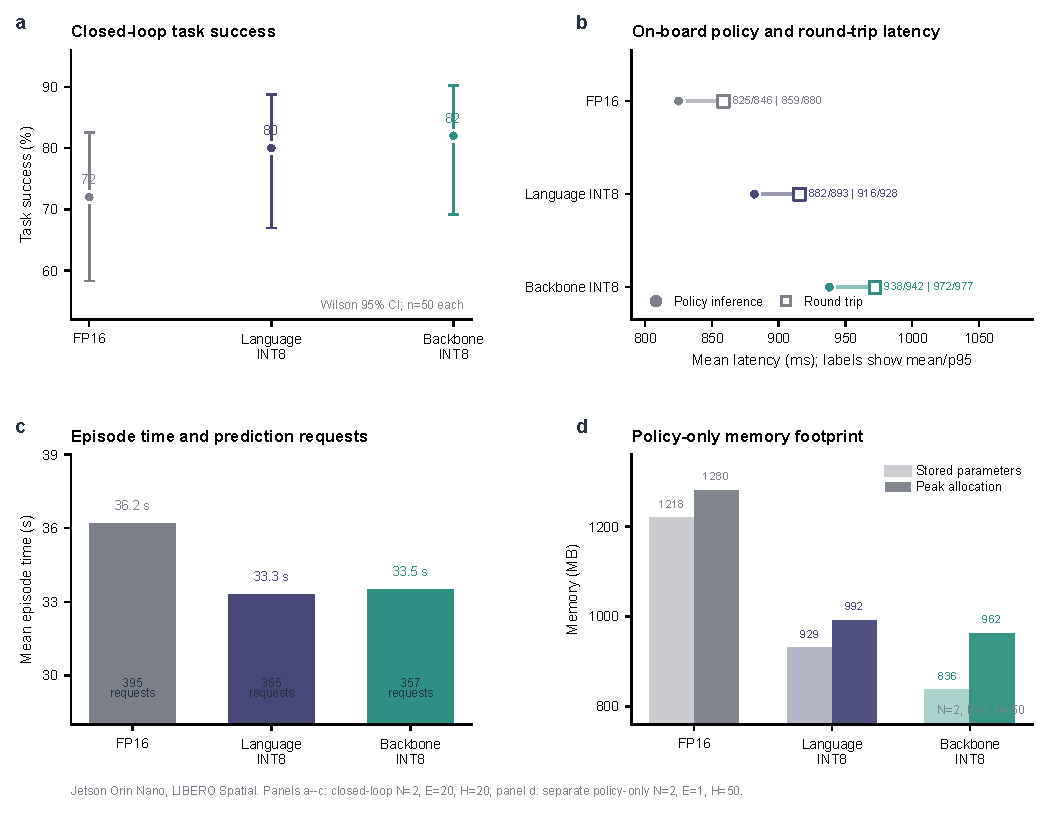
\includegraphics[width=\textwidth]{vla/figures/vla_jetson_onboard_validation.pdf}
  \caption{Jetson on-board validation of selected SmolVLA configurations.
  \textbf{a,} Closed-loop task success with Wilson 95\% confidence intervals.
  \textbf{b,} Policy inference and PC--Jetson round-trip latency; labels show
  mean/p95 values. \textbf{c,} Episode time and prediction-request count.
  \textbf{d,} Separate policy-only parameter storage and peak allocated GPU
  memory. Panels a--c use 50 closed-loop episodes per configuration with
  \((N,E,H)=(2,20,20)\); panel d uses \((2,1,50)\).}
  \label{fig:jetson_onboard_validation}
\end{figure}

\begin{table}
  \centering
  \caption{Jetson on-board validation of selected deployment configurations.
  \textbf{a,} Closed-loop LIBERO Spatial evaluation with
  \((N,E,H)=(2,20,20)\); confidence intervals are Wilson 95\% intervals for
  binary task success. \textbf{b,} Separate policy-only resource benchmark
  with \((N,E,H)=(2,1,50)\); it reports only parameter storage and peak
  allocated GPU memory.}
  \label{tab:jetson_onboard}
  \small
  \setlength{\tabcolsep}{3pt}
  \textbf{a \quad Closed-loop evaluation}\\[-2pt]
  \begin{tabular}{@{}lcccccc@{}}
    \toprule
    Configuration & \shortstack{Success\\(\%)} &
    \shortstack{Wilson 95\%\\CI (\%)} &
    \shortstack{Episode time\\(s)} &
    \shortstack{Inference mean/p95\\(ms)} &
    \shortstack{Round-trip mean/p95\\(ms)} &
    \shortstack{Prediction\\requests} \\
    \midrule
    FP16 baseline & 72.0 & 58.3--82.5 & 36.2 & 825.1 / 846.3 & 858.6 / 879.7 & 395 \\
    Language-only INT8 & 80.0 & 67.0--88.8 & 33.3 & 881.8 / 893.3 & 915.7 / 928.0 & 355 \\
    Backbone INT8 & 82.0 & 69.2--90.2 & 33.5 & 938.1 / 942.5 & 972.2 / 977.2 & 357 \\
    \bottomrule
  \end{tabular}

  \vspace{4pt}
  \textbf{b \quad Policy-only resource benchmark}\\[-2pt]
  \begin{tabular}{@{}lcc@{}}
    \toprule
    Configuration & \shortstack{Stored parameter size\\(MB) \(\downarrow\)} &
    \shortstack{Peak memory\\(MB) \(\downarrow\)} \\
    \midrule
    FP16 baseline & 1217.9 & 1279.7 \\
    Language-only INT8 & 929.4 & 991.8 \\
    Backbone INT8 & 835.9 & 961.8 \\
    \bottomrule
  \end{tabular}
\end{table}

Mean episode time was 36.2\,s for FP16, 33.3\,s for language-only INT8 and
33.5\,s for backbone INT8. The FP16, language-only INT8 and backbone INT8
evaluations generated 395, 355 and 357 prediction requests, respectively.
The shorter INT8 episode times should therefore be interpreted as rollout-level
outcomes rather than evidence of faster individual policy calls.

The separate policy-only resource benchmark measured parameter storage and peak
allocated GPU memory at \((N,E,H)=(2,1,50)\). Relative to FP16, language-only
INT8 reduced stored parameter size from 1217.9 to 929.4\,MB and peak memory
from 1279.7 to 991.8\,MB, reductions of 23.7\% and 22.5\%, respectively.
Backbone INT8 reduced these values to 835.9 and 961.8\,MB, corresponding to
reductions of 31.4\% and 24.8\%. Extending quantisation from the language
transformer to the full vision--language backbone therefore produced a further
10.1\% reduction in stored parameters but only a 3.0\% reduction in peak
allocation, while increasing formal closed-loop mean inference latency from
881.8 to 938.1\,ms. FP16 was retained as the lowest-latency on-board baseline,
language-only INT8 was carried forward into the connector-hybrid ablation, and
backbone INT8 was retained as the broader-scope quantisation boundary. These
measurements characterised a
memory--latency trade-off rather than hardware-native INT8 acceleration.


\subsubsection{Jetson Component-Level Hardware Acceleration (YH)}

TensorRT execution was feasible at the isolated connector and vision-encoder
boundaries, although the available measurements did not support a general
TensorRT speed-up claim for the complete policy. Table~\ref{tab:jetson_hardware}
reports the exact engine measurements, while
Fig.~\ref{fig:vla_hardware_acceleration} relates them to their integration
outcomes. The standalone
256-token connector engine occupied 22.5\,MiB and recorded mean and
95th-percentile GPU latencies of 0.443 and 0.598\,ms, respectively. The
1,024-token connector engine used in the closed-loop hybrid path recorded
0.819\,ms mean latency and 1.116\,ms p95 latency. The standalone FP16 vision
engine, evaluated with a \(256\times256\) input, recorded mean and p95 latencies
of 15.37 and 16.89\,ms. Because the connector measurements used different token
lengths and none of the engines had a matched PyTorch component baseline, these
values characterise executable component paths rather than TensorRT speed-ups.

\begin{table}
  \centering
  \caption{Jetson component-level hardware measurements (n.r., not
  recorded). TensorRT rows with different input specifications are not direct
  speed-up comparisons.}
  \label{tab:jetson_hardware}
  \small
  \setlength{\tabcolsep}{4pt}
  \textbf{a \quad TensorRT component engines}\\[-2pt]
  \begin{tabular}{@{}llrrrr@{}}
    \toprule
    Component & Precision and input &
    \shortstack{Engine size\\(MiB)} &
    \shortstack{Mean\\(ms) \(\downarrow\)} &
    \shortstack{p95\\(ms) \(\downarrow\)} &
    \shortstack{Throughput\\(qps) \(\uparrow\)} \\
    \midrule
    Connector probe & FP16; 256 tokens & 22.5 & 0.443 & 0.598 & 3031.32 \\
    Connector hybrid & FP16; 1,024 tokens & n.r. & 0.819 & 1.116 & 1995.87 \\
    Vision encoder & FP16; \(256\times256\) & 330.9 & 15.37 & 16.89 & 64.98 \\
    \bottomrule
  \end{tabular}

  \vspace{4pt}
  \textbf{b \quad CUDA Graph replay on the FP16 vision engine}\\[-2pt]
  \begin{tabular}{@{}lrrrr@{}}
    \toprule
    Mode &
    \shortstack{Mean\\(ms) \(\downarrow\)} &
    \shortstack{p95\\(ms) \(\downarrow\)} &
    \shortstack{Enqueue\\(ms) \(\downarrow\)} &
    \shortstack{Throughput\\(qps) \(\uparrow\)} \\
    \midrule
    Eager enqueue & 15.44 & 17.31 & 1.2700 & 64.65 \\
    CUDA Graph replay & \textbf{14.50} & \textbf{16.09} & \textbf{0.0145} & \textbf{68.90} \\
    \bottomrule
  \end{tabular}
\end{table}

CUDA Graph replay provided a matched comparison on the same fixed-shape FP16
vision engine. Relative to eager enqueue, graph replay reduced mean GPU latency
from 15.44 to 14.50\,ms and p95 latency from 17.31 to 16.09\,ms, reductions of
6.1\% and 7.0\%, respectively. Enqueue time decreased from 1.2700 to
0.0145\,ms, corresponding to an 87.6-fold reduction in host-side submission
overhead, while throughput increased from 64.65 to 68.90 queries per second.
These gains apply to replay of the fixed-shape vision engine and were not
extrapolated to the dynamic full-policy execution path.

Closed-loop reintegration exposed a narrower deployment boundary than the
standalone component benchmarks. The 1,024-token connector engine was
successfully reintegrated into the complete policy; its task-level effect is evaluated
in Section~4.5. In contrast, loading the FP16 vision engine alongside the full
PyTorch policy failed because the additional engine could not be allocated in
the available GPU/CMA memory. A \(512\times512\)-input INT8 vision engine
calibrated with 400
LIBERO images completed the hybrid path, but the available formal run
summary recorded only 16.0\% task success, a mean episode time of 57.4\,s and a
mean policy-inference latency of 933.6\,ms. This configuration was therefore not
retained for the final ablation. Direct full-policy TensorRT export did not
produce an executable engine, and full-policy CUDA Graph capture was prevented
by dynamically created attention masks, CPU scalar construction and the Python
flow-matching loop. The hardware experiments consequently established
component-level execution and a successful connector integration, rather than a
fully compiled SmolVLA runtime.

\begin{figure}[!t]
  \centering
  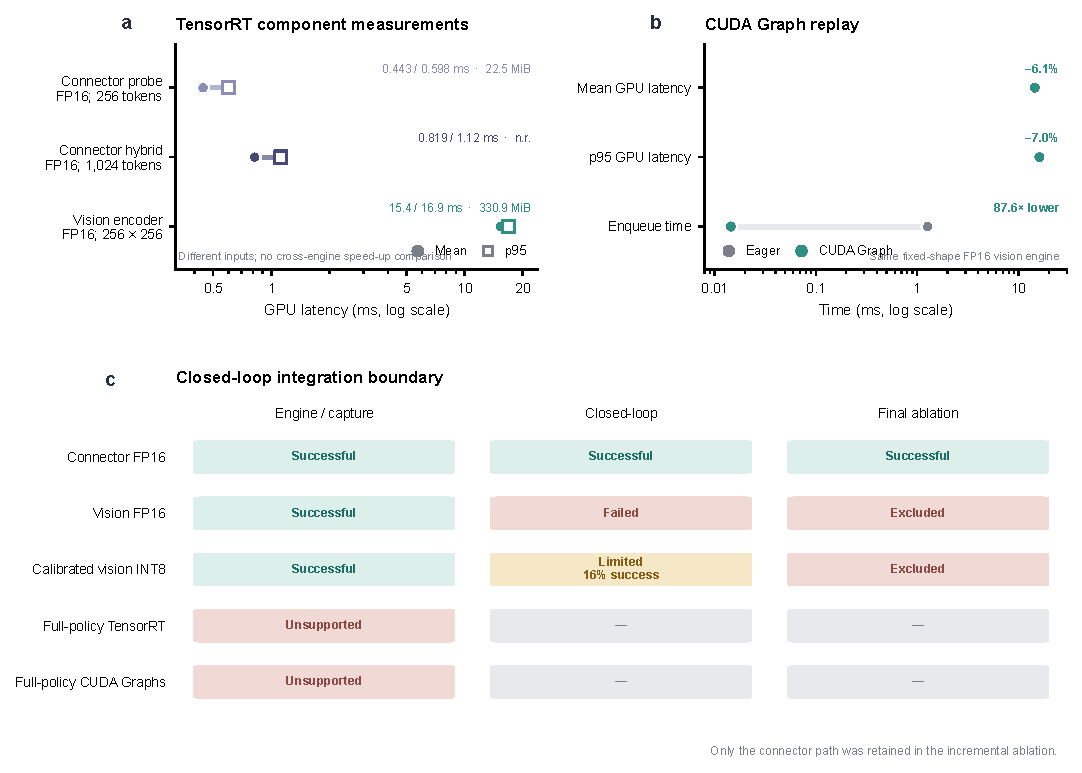
\includegraphics[width=\textwidth]{vla/figures/vla_hardware_acceleration.pdf}
  \caption{Jetson component-level hardware acceleration.
  \textbf{a,} FP16 TensorRT engine measurements by input specification.
  \textbf{b,} Paired eager and CUDA Graph execution on the same FP16 vision
  engine. \textbf{c,} Closed-loop integration outcomes.}
  \label{fig:vla_hardware_acceleration}
\end{figure}

% [VERIFY BEFORE SUBMISSION] The calibrated INT8 vision hybrid values are
% currently available only in the consolidated run summary; archive the raw
% eval_info.json and request-level log before adding confidence intervals or
% request-distribution claims.

\subsubsection{Incremental On-Board Ablation (YH)}

The incremental ablation tested whether the component-level TensorRT connector
remained compatible with the selected software and quantisation settings after
closed-loop reintegration. Under the common 50-episode protocol,
the FP16 baseline, language-only INT8 policy and language-only INT8 policy with
the TensorRT connector achieved task-success point estimates of 72.0\%, 80.0\%
and 76.0\%, respectively (Table~\ref{tab:jetson_ablation} and
Fig.~\ref{fig:vla_incremental_ablation}). Their Wilson 95\%
confidence intervals were 58.3--82.5\%, 67.0--88.8\% and 62.6--85.7\%.
The intervals overlapped across all three configurations and did not support
attributing a task-success change to connector reintegration. The point
estimates likewise did not establish an improvement in task capability.

\begin{table}
  \centering
  \caption{Incremental closed-loop ablation on the Jetson Orin Nano.
  Each configuration used \((N,E,H)=(2,20,20)\) and 50 LIBERO Spatial
  episodes.}
  \label{tab:jetson_ablation}
  \small
  \setlength{\tabcolsep}{4pt}
  \begin{tabular}{@{}lccccc@{}}
      \toprule
      Configuration &
      \shortstack{Success\\(\%) \(\uparrow\)} &
      \shortstack{Wilson 95\%\\CI (\%)} &
      \shortstack{Mean inference\\(ms) \(\downarrow\)} &
      \shortstack{Episode time\\(s) \(\downarrow\)} &
      \shortstack{Prediction\\requests} \\
      \midrule
      Software FP16 & 72.0 & 58.3--82.5 & 825.1 & 36.2 & 395 \\
      Software + language INT8 & 80.0 & 67.0--88.8 & 881.8 & 33.3 & 355 \\
      \shortstack[l]{Software + language INT8 +\\TensorRT connector}
        & 76.0 & 62.6--85.7 & 854.2 & 35.0 & 379 \\
      \bottomrule
  \end{tabular}
\end{table}

The corresponding policy-inference measurements showed a limited latency
recovery rather than a cumulative end-to-end speed-up. Language-only INT8
increased mean inference latency from 825.1 to 881.8\,ms relative to FP16, an
increase of 6.9\%. Replacing the PyTorch connector with its TensorRT engine
reduced this value to 854.2\,ms, 3.1\% below language-only INT8 but still 3.5\%
above FP16. Mean episode times were 36.2, 33.3 and 35.0\,s, while the runs
generated 395, 355 and 379 prediction requests, respectively. Episode time and
request count varied with rollout length and the time at which each task
terminated; they were therefore retained as closed-loop outcomes rather than
interpreted as measurements of individual engine speed.

The ablation consequently supported closed-loop compatibility and partial
recovery of the quantised policy's inference overhead. The smaller change in
full-policy latency than in the standalone connector measurement was consistent
with the connector accounting for only one component of the complete execution
path. The combined configuration neither surpassed the FP16 inference baseline
nor constituted a fully hardware-accelerated policy, because the vision encoder,
text model and action expert remained outside the TensorRT connector boundary.

\begin{figure}
  \centering
  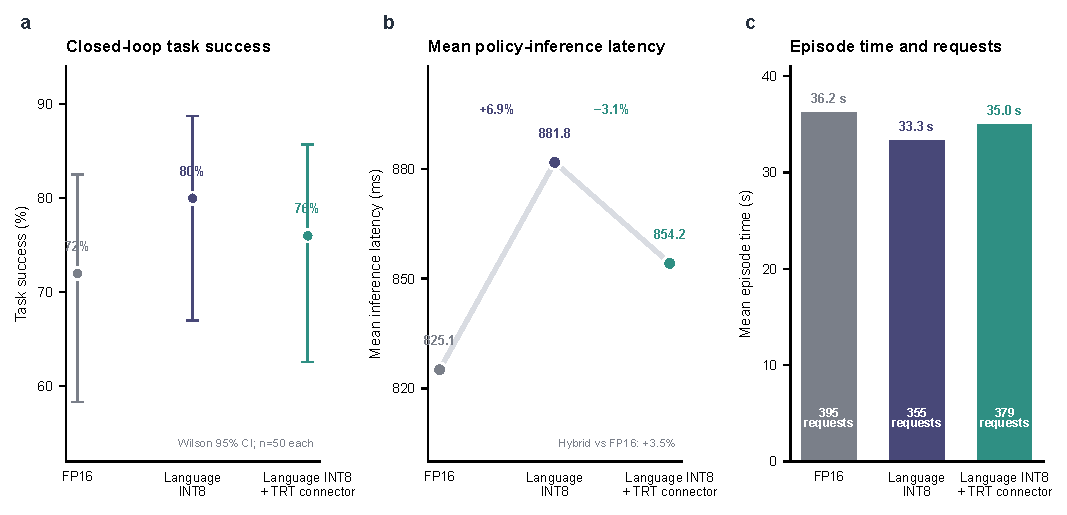
\includegraphics[width=\textwidth]{vla/figures/vla_incremental_ablation.pdf}
  \caption{Incremental on-board ablation.
  \textbf{a,} Task success with Wilson 95\% confidence intervals.
  \textbf{b,} Mean policy-inference latency and adjacent configuration changes.
  \textbf{c,} Mean episode time with prediction-request counts.}
  \label{fig:vla_incremental_ablation}
\end{figure}

% [VERIFY BEFORE SUBMISSION] The connector-hybrid row is currently available
% only in final_ablation_summary.csv. Archive its eval_info.json and
% remote_transport.jsonl before adding p95 or per-task distribution claims.


% [PARTIAL] Restore this heading after Section 4.5 and the final evidence audit.
% \subsection{Conclusion and Future Work}

\clearpage
